

\documentclass[a1paper,portrait,fontscale=0.554]{baposter}

\usepackage[font=small,labelfont=bf]{caption} % Required for specifying captions to tables and figures
\usepackage{booktabs} % Horizontal rules in tables
\usepackage{relsize} % Used for making text smaller in some places
\usepackage{multirow}
\usepackage{pgf}
\usepackage{multicol}
\usepackage{paralist}
\usepackage{color}
\usepackage{subfigure}
\usepackage{lipsum}
\usepackage[normalem]{ulem}
\usepackage{amsmath,amssymb}
\usepackage{mathtools}
\usepackage{tikz}
\usepackage{palatino}
\usepackage{cmap} 
\usepackage{caption}
\usetikzlibrary{shapes,arrows}
\setcounter{totalnumber}{10}
\setcounter{topnumber}{10}
\usepackage{ dsfont }


%% Поиск русских слов в pdf
\usepackage[T2A]{fontenc}             %% Внутренняя кодировка шрифта
\usepackage[utf8]{inputenc}           %% Кодировка исходного текста
\usepackage[english,russian]{babel}   %% Поддержка русского текста

\IEEEoverridecommandlockouts

\usepackage{graphicx}
\usepackage{amsmath}
\usepackage{amssymb}
\usepackage{color}

\usepackage{algorithm}
\usepackage{algpseudocode}
\algnewcommand\algorithmicinput{\textbf{Input:}}
\algnewcommand\INPUT{\item[\algorithmicinput]}
\algnewcommand\algorithmicoutput{\textbf{Output:}}
\algnewcommand\OUTPUT{\item[\algorithmicoutput]}

\usepackage{mathtools}
\DeclarePairedDelimiter{\ceil}{\lceil}{\rceil}
\DeclarePairedDelimiter{\floor}{\lfloor}{\rfloor}

\newcommand{\Fig}[1]{Fig.~\textup{\ref{#1}}}
\graphicspath{{figures/}}
%\usepackage{subcaption}

\newtheorem{definition}{Definition}
\newtheorem{lemma}{Lemma}
\newtheorem{theorem}{Theorem}
\newtheorem{corollary}{Corollary}
\newtheorem{remark}{Remark}
\newtheorem{example}{Example}

\newcommand{\F}{\mathbb{F}}
%\newcommand{\cC}{\mathcal{C}}
%\newcommand{\cR}{\mathcal{R}}
\DeclareMathOperator{\Cl}{Cl} 
\newcommand{\remove}[1]{}

\def\thesubsection{\thesection-\Alph{subsection}}
\def\supp{\qopname\relax{no}{sp}}
\def\avg{{\text{\sf E}}}
\def\sgn{\qopname\relax{no}{sgn}}
\def\rank{\qopname\relax{no}{rk}}
\def\shape{\qopname\relax{no}{shape}}
%\def\wt{\qopname\relax{no}{w}}
\def\proj{\qopname\relax{no}{proj}}
\def\Clap{\qopname\relax{no}{Cap}}
\def\Vol{\qopname\relax{no}{Vol}}
\def\arcsec{\qopname\relax{no}{arcsec}}
\def\argmax{\qopname\relax{no}{argmax}}
\def\gauss{\atopwithdelims []}
\newcommand{\ceilenv}[1]{\left\lceil #1 \right\rceil}
\newcommand{\floorenv}[1]{\left\lfloor #1 \right\rfloor}
\newcommand{\logasymp}{\cong}%\stackrel{\text{\tiny\rm exp}}{\sim}}
\newcommand\nc\newcommand
\nc\bfa{{\boldsymbol a}}\nc\bfA{{\bf A}}\nc\cA{{\mathcal A}}
\nc\bfb{{\boldsymbol b}}\nc\bfB{{\bf B}}\nc\cB{{\mathcal B}}
\nc\bfc{{\boldsymbol c}}\nc\bfC{{\bf C}}\nc\cC{{\mathcal C}}
\nc\bfd{{\boldsymbol d}}\nc\bfD{{\bf D}}\nc\cD{{\mathcal D}}
\nc\bfe{{\boldsymbol e}}\nc\bfE{{\bf E}}\nc\cE{{\mathcal E}}
\nc\bff{{\boldsymbol f}}\nc\bfF{{\bf F}}\nc\cF{{\mathcal F}}
\nc\bfg{{\boldsymbol g}}\nc\bfG{{\bf G}}\nc\cG{{\mathcal G}}
\nc\bfh{{\boldsymbol h}}\nc\bfH{{\bf H}}\nc\cH{{\mathcal H}}
\nc\bfi{{\boldsymbol i}}\nc\bfI{{\bf I}}\nc\cI{{\mathcal I}}
\nc\bfj{{\boldsymbol j}}\nc\bfJ{{\bf J}}\nc\cJ{{\mathcal J}}
\nc\bfk{{\boldsymbol k}}\nc\bfK{{\bf K}}\nc\cK{{\mathcal K}}
\nc\bfl{{\boldsymbol l}}\nc\bfL{{\bf L}}\nc\cL{{\mathcal L}}
\nc\bfm{{\boldsymbol m}}\nc\bfM{{\bf M}}\nc\cM{{\mathcal M}}
\nc\bfn{{\boldsymbol n}}\nc\bfN{{\bf N}}\nc\cN{{\mathcal N}}
\nc\bfo{{\boldsymbol o}}\nc\bfO{{\bf O}}\nc\cO{{\mathcal O}}
\nc\bfp{{\boldsymbol p}}\nc\bfP{{\bf P}}\nc\cP{{\mathcal P}}
\nc\bfq{{\boldsymbol q}}\nc\bfQ{{\bf Q}}\nc\cQ{{\mathcal Q}}
\nc\bfr{{\boldsymbol r}}\nc\bfR{{\bf R}}\nc\cR{{\mathcal R}}
\nc\bfs{{\boldsymbol s}}\nc\bfS{{\bf S}}\nc\cS{{\mathcal S}}
\nc\bft{{\boldsymbol t}}\nc\bfT{{\bf T}}\nc\cT{{\mathcal T}}
\nc\bfu{{\boldsymbol u}}\nc\bfU{{\bf U}}\nc\cU{{\mathcal U}}
\nc\bfv{{\boldsymbol v}}\nc\bfV{{\bf V}}\nc\cV{{\mathcal V}}
\nc\bfw{{\boldsymbol w}}\nc\bfW{{\bf W}}\nc\cW{{\mathcal W}}
\nc\bfx{{\boldsymbol x}}\nc\bfX{{\bf X}}\nc\cX{{\mathcal X}}
\nc\bfy{{\boldsymbol y}}\nc\bfY{{\bf Y}}\nc\cY{{\mathcal Y}}
\nc\bfz{{\boldsymbol z}}\nc\bfZ{{\bf Z}}\nc\cZ{{\mathcal Z}}
\nc\od{{\bar d}}\nc\ow{{\bar w}}\nc\odelta{{\bar\delta}}
\nc\ox{{\bar x}}\nc\oy{{\bar y}}\nc\ou{{\bar u}}
\nc\oh{{\bar h}}
\DeclareMathOperator{\E}{\text{\sf E}} 
\DeclareMathOperator{\ent}{h} 
\usetikzlibrary{positioning}

\graphicspath{{figures/}} % Directory in which figures are stored

\definecolor{bordercol}{RGB}{124,195,254} % Border color of content boxes
\definecolor{headercol1}{RGB}{140,201,255}%204,255,204} % Background color for the header in the content boxes (left side)
\definecolor{headercol2}{RGB}{55,88,148} % Background color for the header in the content boxes (right side)
\definecolor{headerfontcol}{RGB}{0,0,0} % Text color for the header text in the content boxes
\definecolor{boxcolor}{RGB}{255,255,255} % Background color for the content in the content boxes


\definecolor{mygreen}{RGB}{218,249,281}
\definecolor{myblue}{RGB}{25,120,150}

\newcommand\reduline{\bgroup\markoverwith
{\textcolor{red}{\rule[0.5ex]{2pt}{0.8pt}}}\ULon}

\newcounter{mybox}
\newcommand\tikzmark[1]{%
\tikz[remember picture,overlay] \node[inner xsep=0pt] (#1) {};
}
\newcommand\ColorBox[2][]{%
\stepcounter{mybox}%
\node[draw=red!70!black,thick,fill=red!20,align=center,#1] (box\themybox) {#2};
}

\newcommand{\DQoS}{D^{QoS}}
\newcommand{\PLRQoS}{PLR^{QoS}}
\newcommand{\Dres}{\ensuremath{D^{res}}}
\newcommand{\Tres}{\ensuremath{T^{res}}}
\newcommand{\Tin}{\ensuremath{T^{in}}}
\newcommand{\Tout}{\ensuremath{T^{out}}}
\newcommand{\tres}{\ensuremath{t^{res}}}
\newcommand{\tin}{\ensuremath{t^{in}}}
\newcommand{\tout}{\ensuremath{t^{out}}}
\newcommand{\Iout}{\ensuremath{I^{out}}}
\newcommand{\Iin}{\ensuremath{I^{in}}}
\newcommand{\Idis}{\ensuremath{I^{dis}}}
\newcommand{\load}{\eta}


\newcommand{\PER}{\ensuremath{q}}
\newcommand{\Qmax}{\ensuremath{Q^{max}}}

\newcommand{\pin}{\ensuremath{p^{in}}}
\newcommand{\Pin}{\ensuremath{P^{in}}}
\newcommand{\pout}{\ensuremath{p^{out}}}
\newcommand{\Pout}{\ensuremath{P^{out}}}


\renewenvironment{itemize}[1]{\begin{compactitem}#1}{\end{compactitem}}
\renewenvironment{enumerate}[1]{\begin{compactenum}#1}{\end{compactenum}}
\renewenvironment{description}[0]{\begin{compactdesc}}{\end{compactdesc}}

\begin{document}



\begin{poster}{
grid=false,
columns=2,
borderColor=bordercol, % Border color of content boxes
headerColorOne=headercol1, % Background color for the header in the content boxes (left side)
headerColorTwo=headercol2, % Background color for the header in the content boxes (right side)
headerFontColor=headerfontcol, % Text color for the header text in the content boxes
boxColorOne=boxcolor, % Background color for the content in the content boxes
headershape=roundedright, % Specify the rounded corner in the content box headers
headerfont=\Large\sf\bf, % Font modifiers for the text in the content box headers
textborder=rectangle,
background=none,
headerborder=open, % Change to closed for a line under the content box headers
boxshade=plain
}
{}
%
%----------------------------------------------------------------------------------------
%	TITLE
%----------------------------------------------------------------------------------------
%
{\sf\bf  Сравнение\ \ \ методов\ \ \ построения\ \ \ полярных\ \ \ кодов\ \ \ для\ \ \ каналов\ \ \ с\ \ \ аддитивным\ \ \ белым \ \ \ гауссовским \ \ \ шумом} 
% Poster title
{\vspace{1em}
\begin{tabular}{c c c c c c c}
Глеб Балицкий &Андрей Дзись &Алексей Фролов &\quad
\\
ИППИ  РАН &\quad ИППИ  РАН &\quad ИППИ  РАН 
\\
МФТИ &\quad МФТИ &\quad Сколтех
\\
gleb.balitskiy@phystech.edu  &\quad  andrey.dzis@phystech.edu  &\quad al.frolov@skoltech.ru

\end{tabular}}

\headerbox{1.Мотивация}{name=1,column=0, span = 1}{

 Полярные коды являются первыми известными кодами с субквадратичной сложностью кодирования и декодирования, для которых доказан факт достижения пропускной способности дискретных двоичных каналов без памяти, например, бинарного канала со стираниями (BEC). Вследствие особенностей построения кода, его структура непосредственно зависит от SNR в канале. Таким образом, актуальной задачей является нахождение таких параметров кода, при которых код может работать на некотором заранее заданном диапазоне SNR.
\centering{\includegraphics[scale=0.4]{1}}
}

\headerbox{2. Полярные коды}{name=2,column=0,span=1, below=1}{ 
Принцип работы полярных кодов построен на явлении поляризации канала. Явление заключается в следующем: мы из набора $N$-независимых копий данного B-DMC канала можем создать второй набор $N$ двоичных каналов $W_N^{(i)}: 1\leq i\leq N$ так, что с увеличением $N$ для $i$, для которых $I(W_N^{(i)})$ стремится к 1, пропускная способность соответствующих каналов достигает $I(W)$.Соответственно, для $i$, для которых $I(W_N^{(i)})$ стремится к 0, достигает значения $1-I(W)$. Таким образом, для передачи достаточно выбирать из этих каналов лишь те,пропускная способность которых стремится к 1. Коды, построенные по данному принципу, называются полярными.

На примере BEC рассмотрим подробнее поляризацию канала, состоящую из двух этапов: объединение  и разделение канала.
В объединении основная задача рекурсивно получить вектор $W_N:\mathcal{X}^N \rightarrow \mathcal{Y}^N$. Рекурсия начинается с $n = 0$ (нулевой шаг рекурсии) с единственной копией канала $W$ и $W_1 \triangleq W$ Первый шаг $n = 1$ начинается с двух независимых копий $W_1$ и составляет $W_2: \mathcal{X}^2 \rightarrow \mathcal{Y}^2$ (см.рис.1) с вероятностью ошибки:
\begin{equation}
    W_2(y_1,y_2|u_1,u_2) = W(y_1|u_1 \oplus u_2)W(y_2|w_2)
\end{equation}
\tikzset{%
  block/.style    = {draw, thick, rectangle, minimum height = 3em,
    minimum width = 3em},
  sum/.style      = {draw, circle, node distance = 2cm}, % Adder
  input/.style    = {coordinate}, % Input
  output/.style   = {coordinate} % Output
}
% Defining string as labels of certain blocks.
\newcommand{\suma}{\Large$+$}
\newcommand{\inte}{$\displaystyle \int$}


\caption{}
\\

В результате входной вектор $u_1^N$ преобразуется в вектор $s_1^N$ так, что $s_{2i-1} = u_{2i-1} \oplus u_{2i}$, $s_{2i}=u_{2i} $
\\
Разделение канала заключается в делении $W_N$ в последовательность $N$ бинарных каналов $W_(i)^N : \mathcal{X} \rightarrow \mathcal{Y}^N \times \ \mathcal{X}^{i-1}, 1\leq i \leq N$ с пропускными способностями:
\begin{equation}
    W_N^{(i)}(y_1^N,u_1^{i-1}|u_i) \triangleq \sum\limits_{u^N_{i+1} \in\mathcal{X}^{N-i}} \frac{1}{2^{N-1}}W_N(y_1^N|u_1^N)
\end{equation}
\\ 
Построение кода будем производить над двоичным полем $GF(2)$. Для двух векторов $a_1^N$ и $b_1^N$ через $a_1^N \oplus b_1^N$ обозначим покомпонентное суммирование по модулю 2. 
%Для матриц $A=[A_{ij}]$ размерности $m \times n$ и $B=[B_{ij}]$ размерности $r \times s$ произведение Кронекера определяется как:
%\begin{equation}
%    A\otimes B = \begin{bmatrix}
%A_{11}B & \cdots & A_{1n}B \\
%\vdots & \ddots & \vdots \\
%A_{m1}B & \cdots & A_{mn}B
%\end{bmatrix} 
%\end{equation}
%матрица размерности $mr \times ns$. 

Степень $A^{\otimes n}$ определяется как $A \otimes A^{\otimes (n-1)}$  для $n \geq 1$. Для $n = 0$ определим $A^{\otimes 0} \triangleq [1]$.
Пусть на вход кодера подается последовательность векторов $x^N_1$ длины $N = 2^n$, тогда, обозначая последовательность кодовых слов $u_1^N$, получаем равенство:
\begin{equation}
    x^N_1 = u_1^NG_N
\end{equation}
где $G_N$ порождающая матрица, равная:
\begin{equation}
    G_N = B_N F^{\otimes n}
\end{equation}
где $B_N$ матрица перестановки, а $F^{\otimes n} = F \otimes F^{\otimes (n-1)}$, где $F \triangleq  \begin{bmatrix}
1  & 0  \\
1  & 1 \\
\end{bmatrix} $

}

\headerbox{3. Гауссовский канал}{name=3,column=0,span=1, below=2}{
В данной работе рассмотрен канал с аддитивным белым гауссовским шумом (АБГШ). Предполагается, что шум имеет нулевое среднее и двустороннюю спектральную плотность $\sigma^2 $.
В канале аддитивный шум $n(t)$  прибавляется к сигналу $s(t)$. То есть на выходе канала мы имеем сигнал $s_{out}(t)$ равный:
\begin{equation}
    s_{out}(t)=s(t)+n(t)
\end{equation}
}

\headerbox{4. Методы построения}{name=4,column=0,span=1,below=3}{

Вначале рассмотрим метод построения полярного кода на основе оценки параметров Бхаттачариa. Было доказано, что для каждого виртуального канала параметр Бхаттачариa является верхней границей для вероятности ошибки в этом канале.  
\\

Для построения кода нужно выбрать каналы с наименьшими значениями параметра. Так как точный расчет этих параметров очень сложен, мы решили воспользоваться оценкой сверху, а именно:
\\
\begin{equation}
    Z(W^{(2i-1)}_{2N}) \leq 2Z(W^{(i)}_N) - Z(W^{(i)}_N)^{2}
\end{equation}
\begin{equation}
    Z(W_{2N}^{(2i)}) = Z(W^{(i)}_N)^2
\end{equation}

Второй метод заключается в оценке вероятности ошибки в каждом виртуальном канале, используя Гауссовскую аппроксимацию, и выборе каналов с минимальной ошибкой. Вероятность ошибки можно оценить с помощью формул, представленных ниже: 
\begin{equation}
    E[L^{(2i-1)}_n] = \phi^{-1}(1-(1-\phi(E[L^{(i)_{n/2}}]))^2)
\end{equation}
где:
\begin{equation}
\phi(x) = 
 \begin{cases}
   1 - \frac{1}{\sqrt{4\pi x}}\int_{-\infty}^{\infty}\tanh{\frac{u}{2}}e^{-\frac{(u-x)^2}{4x}}dx &\text{ $x > 0 $}\\
   1 &\text{$x=0$}
 \end{cases}
\end{equation}
\begin{equation}
    E[L^{(2i)}_{n}] = E[L^{(i)}_{n/2}]
\end{equation}
\begin{equation}
    \pi_i \approx Q \Bigg(\sqrt{E[L^{(i)}_{n/2}]/2})\Bigg), 1 \leq i \leq n
\end{equation}
где:
\begin{equation}
    L_1^{(i)}(y_i) \sim  \mathcal{N}(\frac{2}{\sigma^2},\frac{4}{\sigma^2})
\end{equation}
\begin{equation}
    L_{i} = \ln{\frac{\mathds{P}(y_i|0)}{\mathds{P}(y_i|1)}}
\end{equation}
\\
- логарифмическое отношение правдоподобия 

}

\headerbox{5. Численные результаты}{name=upper,column=1}{
Для исследования метода на основе оценки параметров Бхаттачариa были рассмотрены кодовые слова с длиной $ N = 512$ на трех скоростях: $R = 0.25$, $R = 0.5$, $R = 0.75$. 
\begin{center}
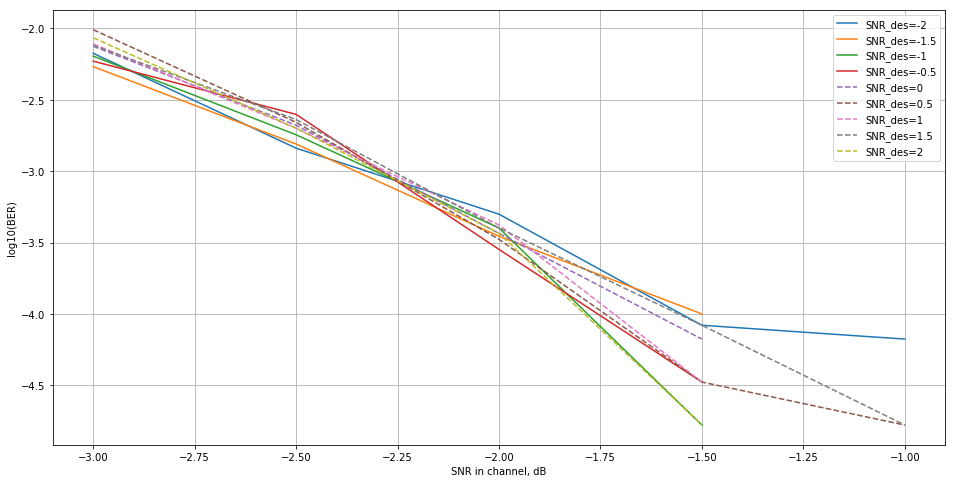
\includegraphics[width=0.5\linewidth]{BAT_0_25}
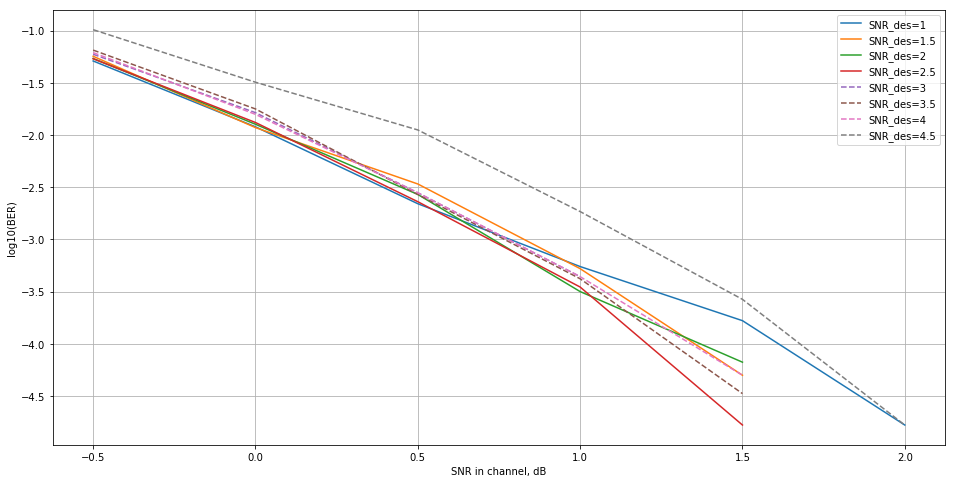
\includegraphics[width=0.5\linewidth]{BAT_0_5}
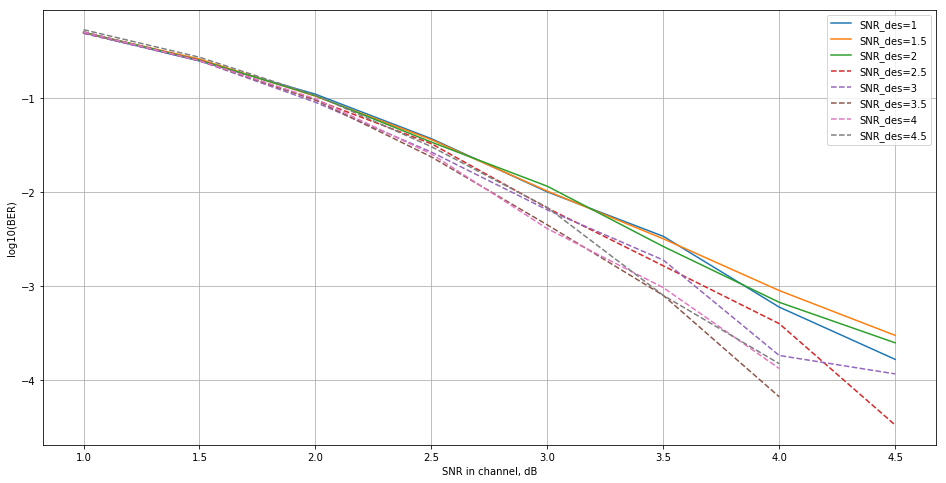
\includegraphics[width=0.5\linewidth]{BAT_0_75}
\caption{подпись к рисунку}
\end{center}
Исследуя полученные зависимости, можно сделать выводы:
\\
1) $R=0.25$: Самая эффективная оптимизация кода на $ SNR_{opt} =-1$
\\
2) $R=0.5$:  Самая эффективная оптимизация кода на $ SNR_ {opt} = 2.5$
\\
3) $R=0.75$: Самая эффективная оптимизация кода на $ SNR_{opt} = 3.5$
\\

Для метода на основе оценки вероятности ошибки аналогично были рассмотрены кодовые слова с длиной $n = 512$ на трех скоростях: $R =  0.25$, $R = 0.5$, $R = 0.75$.
Здесь также видно, что есть определенные значения  параметра  $SNR_{opt}$, при которых код показывает наиболее высокую эффективность:
\\
\begin{center}
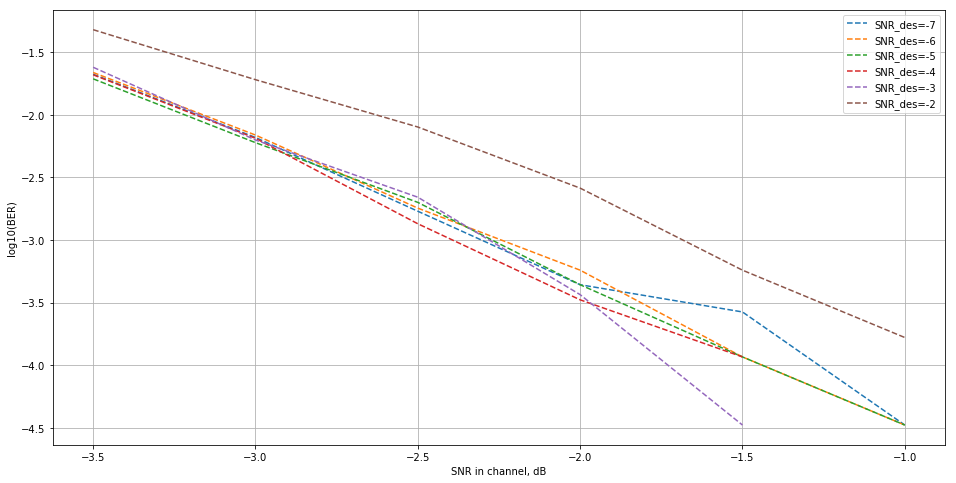
\includegraphics[width=0.5\linewidth]{DE_0_25}
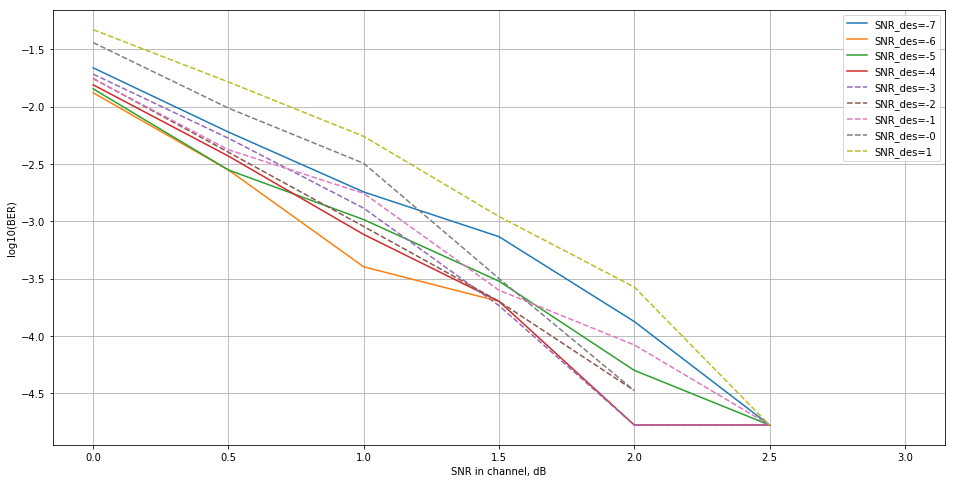
\includegraphics[width=0.5\linewidth]{DE_0_5}
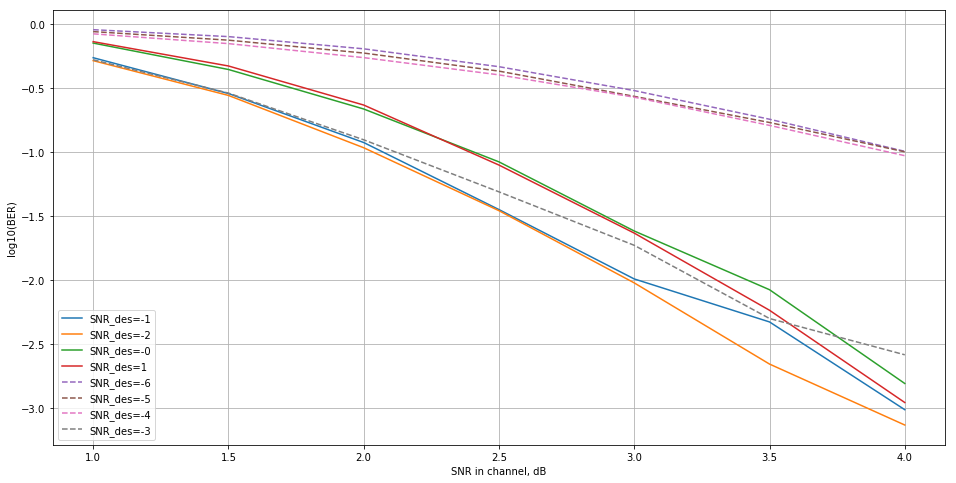
\includegraphics[width=0.5\linewidth]{DE_0_75}
\end{center}
\\
1) $R=0.25$: Самая эффективная оптимизация кода на $ SNR_{opt} = -3$
\\
2) $R=0.5$:  Самая эффективная оптимизация кода на $ SNR_ {opt} = -6$
\\
3) $R=0.75$: Самая эффективная оптимизация кода на $ SNR_{opt} = -2$
\\

Сравнение двух методов:
\begin{center}
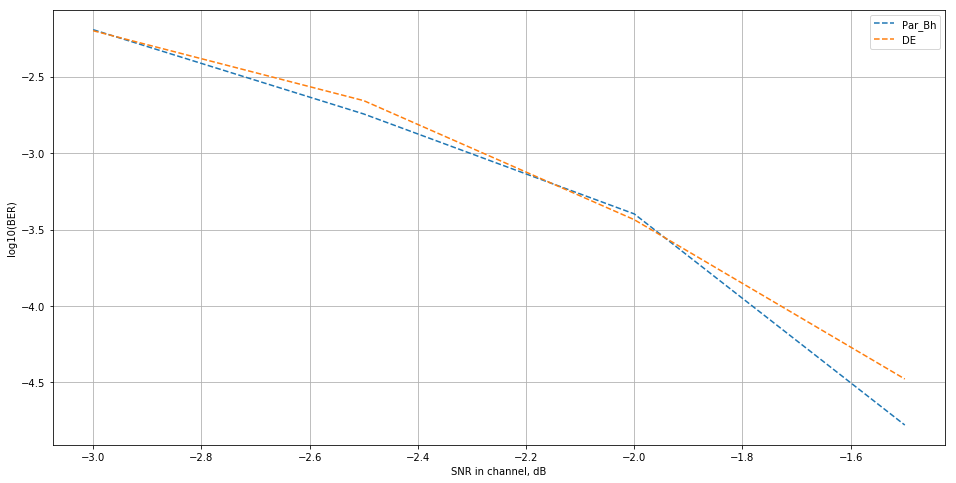
\includegraphics[width=0.49\linewidth]{com_0_25}
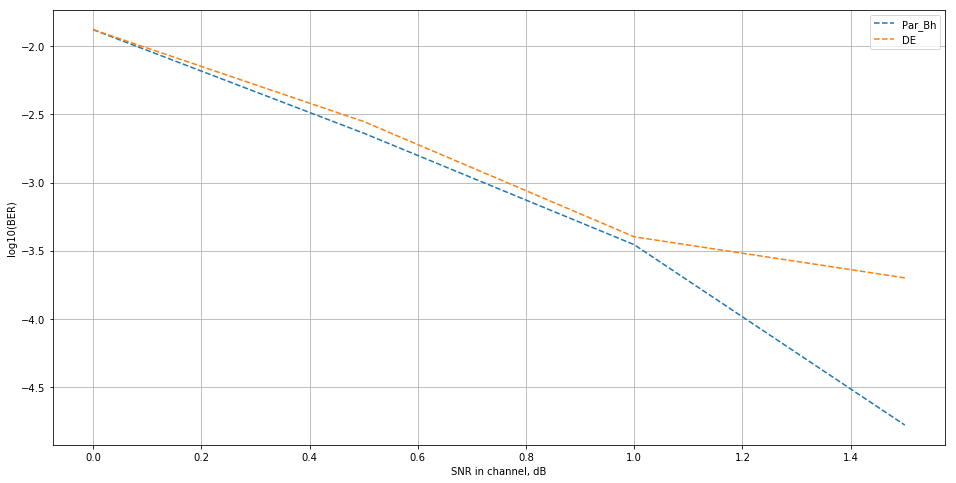
\includegraphics[width=0.49\linewidth]{com_0_5}
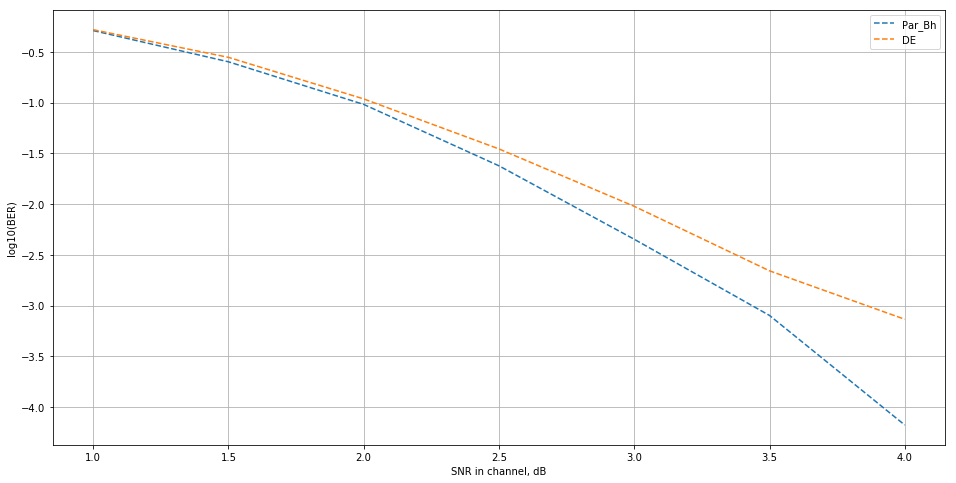
\includegraphics[width=0.449\linewidth]{com_0_75}
\end{center}

}
\end{poster}
\end{document}